\documentclass[12pt]{article}
\usepackage[margin=1in]{geometry}
\geometry{letterpaper}                  
\usepackage{graphicx}
\usepackage[hyphens]{url}
\usepackage{fancyhdr}
%\pagestyle{fancy}
\usepackage{fixltx2e}
\usepackage{amsmath,amsfonts,amsthm,amssymb}
\usepackage{graphicx}
\usepackage{algorithm}
\usepackage{algorithmic}
\usepackage{url}
\usepackage[normalem]{ulem}
\usepackage[pdftex]{color}
\usepackage{varioref}
\usepackage{mathrsfs}
\usepackage{amsmath}
\labelformat{equation}{\textup{(#1)}}
\usepackage[sort&compress,colon,square,numbers]{natbib}
%\usepackage{cite}


\usepackage{color}
\newcommand{\todo}[1]{{\color{red}{\it TODO: #1}}}

\DeclareMathOperator*{\argmin}{arg\,min}


\begin{document}

\begin{center}\Large \bf EN.580.694: Statistical Connectomics \\ Final Project Report \end{center}
\begin{center} Michael Norris $\cdot$  \today \end{center}
\bigskip


\subsection*{Title}
$\\ \\$
\centerline{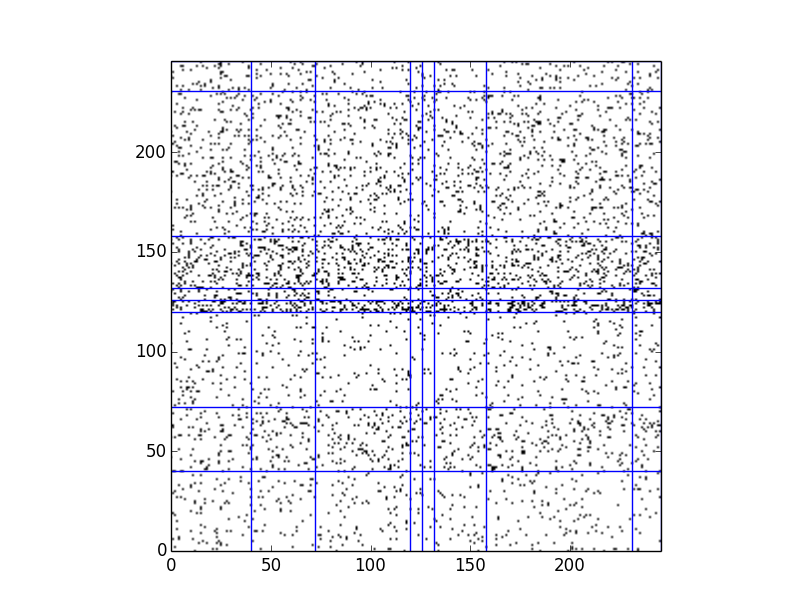
\includegraphics[scale=0.5]{adjacencymatrix.png}}
\newpage

\paragraph{Opportunity}
Graph Models allow us to generate similar graphs from a smaller amount of
parameters.  If we can model connectomes well, then a good model allows us to
generate similar connectomes to perform statistical analysis on similar graphs.
The paper by Pavlovic \cite{pavlovic} used the Erdos Reyni mixture model as an
approximation of the C. Elegans connectome.  Using other graph models to perform
the same analysis will aid future researchers in selecting tools for
connectomics work.

\paragraph{Challenge}

\paragraph{Action}
The Random Dot Product Graph Model (RDPG) represents
\paragraph{Resolution}
Shown above is the TRT result for each atlas using graphs from the KKI2009 dataset. We can see here that with the provided graphs, the Desikan and Harvard-Oxford atlases correctly match $41$ of $42$ scans and have $70$ and $48$ regions, respectively. The Juelich and Talairach atlases both correctly matched all subjects and have $121$ and $1106$ regions, respectively. It can also be seen that the Talairach atlas has much higher discrimination across subjects than the other three atlases, as indicated by the larger dynamic range of image intensities. This suggests that parcelation schemes with too few regions may discard useful information about the brain graphs.
\paragraph{Future Work}
Moving forward, it we will evaluate whether or not specific atlas region labels matter when performing comparing graphs, or rather the scale/number of regions. Randomly permuted atlases could be generated over a large range of scales and a peak operating point determined. This information can aide in building better, more interpretable classifiers for inference and diagnosis.

\newpage

\bibliography{statconn.bib}
\bibliographystyle{plain}


\end{document}  















